\documentclass[11pt]{article}

\usepackage{url}
\usepackage{graphicx}
\usepackage{float}
\setlength{\parskip}{0.5cm plus4mm minus3mm}

\textwidth=6.4in
\textheight=8.5in
\hoffset=-0.7in
\voffset=-0.7in

\setlength{\parindent}{0cm} 


\include{notation}

\hyphenation{Text-Wrangler}

\title{Introduction to localized crustal magnetic field calculations}
\author{Alain Plattner}

\begin{document}
\maketitle

\section{Preparations}

You will either need Matlab or Octave. If you don't have Matlab and you don't want to spend a lot of money you can get Octave for free. If you are using Matlab, you can skip the rest of this section and go straight to section \ref{installing}.

\subsection{Obtaining and installing Octave}

\subsubsection{Mac}

If you are using a Mac, you can follow the instructions from \url{http://wiki.octave.org/Octave_for_MacOS_X}. I recommend manual installation from source. 

First you need to install Apple's developer software XCode. You can get it from Apple's App store. Once you installed XCode, you need to activate the command line tools by opening a terminal and running in the terminal:

\qquad \verb!xcode-select --install!

Now you can install MacPorts. After you installed MacPorts, open a new terminal and run 

\qquad \verb!sudo port install fltk!

You now have two options to install Octave. If you want to use fast computations, then use the following command to install it. Warning: This will increase the installation time by several hours: 

\qquad \verb!sudo port install octave +fltk +atlas +docs!

If you don't need to do large calculations, then you should be fine with the more simple installation:

\qquad \verb!sudo port install octave +fltk +docs!

\subsubsection{Windows}

For Windows you can directly download the installer from

\url{https://www.gnu.org/software/octave/}

 %If you are using Windows I recommend installing Cygwin \url{https://www.cygwin.com/}. During the installation you will be asked which packages you want to add. Make sure you add the packages ``octave'', ``gnuplot'', ``X11'', and ``xinit''.
 
 \subsubsection{Additional components}

You will need a good editor for text files. For Mac I recommend TextWrangler which can be found in \url{http://www.barebones.com/products/textwrangler/}. For Windows I recommend Notepad++ \\ \url{http://notepad-plus-plus.org/}. 

%You can find an introduction to Cygwin on \url{http://www2.imm.dtu.dk/courses/02333/cygwin_tutorial/index.html} and a tutorial for Octave on \url{http://www-mdp.eng.cam.ac.uk/web/CD/engapps/octave/octavetut.pdf}.

%To run Octave in Cygwin you first have to run ``startxwin'' in Cygwin and then start Octave within the new window that opened.

If you are using a Mac and followed the instructions above, you will need to install the IO and the statistics package. Run
%We will require the statistics package in Octave. To install it, in Octave run

\qquad \verb+pkg install io -forge+

and when it's done, run

\qquad \verb+pkg install statistics -forge+

The IO installation might give you some warnings but don't worry, these are just warnings about notations inside the program, nothing that could harm your computer.

If you installed Octave via Cygwin you already have all the packages.

\emph{In the following, whenever I say ``run xxxx'' I mean in Octave or Matlab, type xxxx and press enter.}

\emph{Always before you use an Octave program for example by the name xyz, run ``help xyz'' without the quotation marks to read about what input is required and what the output will be.}

\section{Installing the local crustal field inversion software}\label{installing}

Unpack the zip file in your working folder. you will see a folder structure containing the folders ``datafiles'', ``ext'', ``Plattner'', ``Plattner\_exp'', ``run'', and ``Simons''. The folder ``Simons'' contains programs written by Frederik Simons and most of the programs can be found on his homepage \url{http://geoweb.princeton.edu/people/simons/software.html}. The folder ``Plattner'' contains programs written by Alain Plattner and most of them can be found on the website \url{http://www.princeton.edu/~plattner/software.html}. The folder ``Plattner\_exp'' contains new and unpublished programs by Alain Plattner including programs for localized crustal magnetic field calculations. The folder ``datafiles'' contains repositories in which in-between steps and results for lengthy calculations will be stored. The folder ``run'' is the main folder in which you will be working.

As a first step: initialize the folder structure in ``datafiles'' by going into that folder and running

\qquad \verb+initializefolder+

This should create many folders.

\section{Initialization}

Next go to the folder ``run'' and run

\qquad \verb+setpaths+

This initializes the paths to the folder structure. You will need to do this whenever you start Octave or Matlab and want to work with these programs. The remainder of this section is only for Octave users. Matlab users can skip straight to section \ref{examples}.


We will also need the statistics package, so run 

\qquad \verb+pkg load statistics+

If you are using a Mac, then the standard Octave plotting is not so good.Let's switch it to fltk:

\qquad \verb+graphics_toolkit('fltk')+

If you are using Windows, don't switch but keep it the way it is. If you accidentally switched, you can go back to the standard by running \verb+graphics_toolkit('gunplot')+

When you are displaying a lot of output, Octave usually shows this step by step. This is a bit annoying. We'll turn this off by running

\qquad \verb+more off+

You will need to run all of these initializations every time you start Octave. If you like you can copy-paste the commands into the setpath.m file such that you only need to run ``setpaths''.

\section{First examples}\label{examples}
To get started with the examples, run

\qquad \verb+help examples+

This will show you a description of what the program does. For example, try

\qquad \verb+examples(1)+

This will take a while to calculate. If it takes too long you can abort by pressing ``Ctrl-c''. This might also end your Octave session, so you will need to start Octave again and run ``setpaths'' again. Let's have a look why it takes so long. To do that, open examples.m with your text editor (either Notepad++ or Textwrangler or whichever you would like to use).

You will first see a couple of lines with \verb+%+ 
signs in the beginning. This is the help component of the program. Any later line with a \verb+%+
in the beginning is simply a comment that does not do anything but can be very helpful for anyone who reads the program.

You see that a few lines down there is a comment that says ``Maximum spherical-harmonic degree:''. Underneath this comment is the line ``Lmax=20''. Here, Lmax defines the maximum spherical-harmonic degree. I will give a more detailed explanation about spherical harmonics at a later point but basically: The maximum spherical-harmonic degree defines the resolution of features in our analysis. The larger it is, the more details we see, but also the longer the computations take and the more sensitive we are to noise in the data!

Set Lmax to a lower value. Maybe 10. Save, and then run again

\qquad \verb+examples(1)+

This should first generate the outlines of Africa and then a plot a sphere with some blurry colors on it. You can rotate the sphere by clicking on ``R'' and then rotate with your mouse.

If you now run the example again

\qquad \verb+examples(1)+

you will see that the calculations are much faster. This is because in-between steps were stored.

Congrats, you calculated and plotted your first ``altitude vector Slepian function``. Play around with the other examples. You might need to set the maximum degree to a lower value to make calculations faster, or to a higher value if you want a more realistic and challenging example.

Also, in examples.m a few lines above Lmax you can read ``\% Region'', below that ``\%dom=[170 20];'' and below that ``dom='africa';''. The last, uncommented line defines the region. You can try other named regions such as 'namerica' for North America, or 'samerica', or 'eurasia'. Or you can choose a polar caps for example of opening angle 10 degrees by setting ``dom=10'' or a polar ring by giving it two numbers like ``dom=[20 10];''. It is also possible to run calculations for spherical cap centered somewhere else than the north pole. See the help comments for \verb+glmalphaup.m+, \verb+gradvecglmalphaup.m+, etc. You can even write a wrapper function for a list of lon/lat locations of the outline of your generic region. Generally, spherical caps and rings are much faster to calculate and require much less memory than irregular regions. This is particularly important for very large spherical-harmonic degrees (200 and beyond).

\verb+examples(3)+ and \verb+examples(4)+ are inversions for artificial data with a noise level you can choose. These are the key examples for estimating crustal fields from satellite altitude. In principle you can take these examples (3 for radial component data only and 4 for three component vectorial data), put in your data, select your region, satellite altitude, planet radius, maximum spherical harmonic degree, and number of Slepian functions you want to use, and run it to calculate your crustal magnetic field model.

\section{Introduction to spherical harmonics}

Spherical harmonics are a counterpart to monomials (building blocks of polynomials, the ``wiggly'' lines) but on the sphere. Remember that polynomials were always sums of monomials multiplied by some numbers. For example $3x^2 - 20.95x + 5.11113$ is a \emph{polynomial} consisting of the \emph{monomials} $x^2$, $x$, and $1$ multiplied by the \emph{coefficients} $3, -20.95, 5.1113$ and then summed up. Spherical harmonics do exactly the same. Each of them has a degree, we multiply them with coefficients and then sum them up. One thing that is different is that besides having a degree, spherical harmonics also have an order. This is because they live on a sphere which is a surface and therefore has two directions in which it can ``wiggle''. 

Here we denote spherical harmonics with the capital letter $\Yfun$ followed by its degree $l$ and its order $m$ as indices. Both degree $l$ and order $m$ are integers. The degree $l$ is 0 or greater whereas the order can be positive, zero, or negative. So we generally write $\Yfun_{l\,m}$. For example for degree 4 and order 2 it will be $\Yfun_{4\,2}$ (note the small gap between 4 and 2). The \emph{degree} $l$ of a spherical harmonic says, how many zero-crossing lines it has in total. The \emph{order} $m$ of a spherical harmonic says how many of the zero-crossings are perpendicular to the equator. The sign of the order says if one of the zero-crossings is along the prime-meridian (negative order $m$) or if the maximum value is on the prime meridian (positive order $m$). From this explanation it is clear that the order $m$ must always be equal or smaller to the degree $l$ (there can't be more zero-crossings perpendicular to the equator than there are zero-crossings altogether).

 Let's look at a few examples. To make it easier to visualize the spherical harmonics, I am plotting them on a sphere and in Mollweide projection over Earth's map. $\Yfun_{0\,0}$ is just a constant number over the entire planet. That's a bit boring so I won't plot it here.

\begin{figure}[H]
\centering
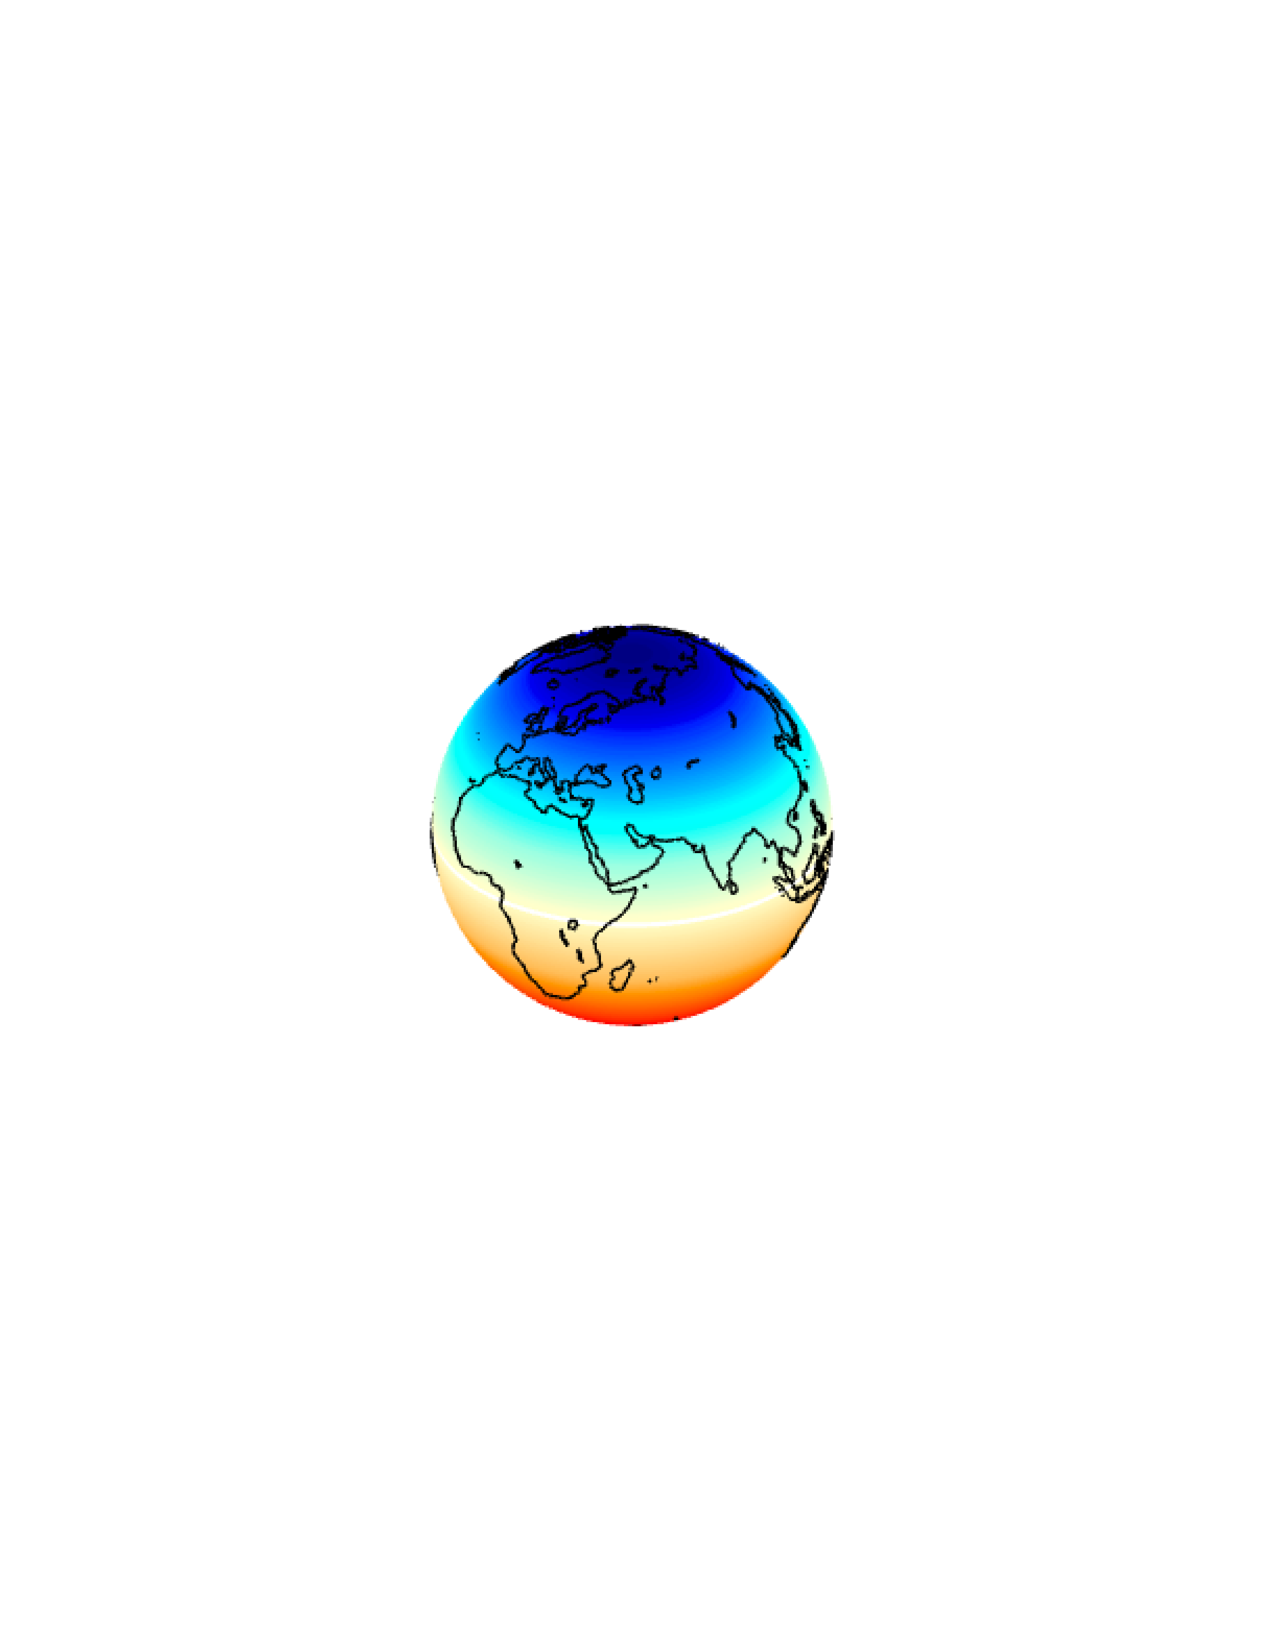
\includegraphics[width=0.4\textwidth,trim = 7cm 10cm 7cm 10cm, clip]{figures/Y10}
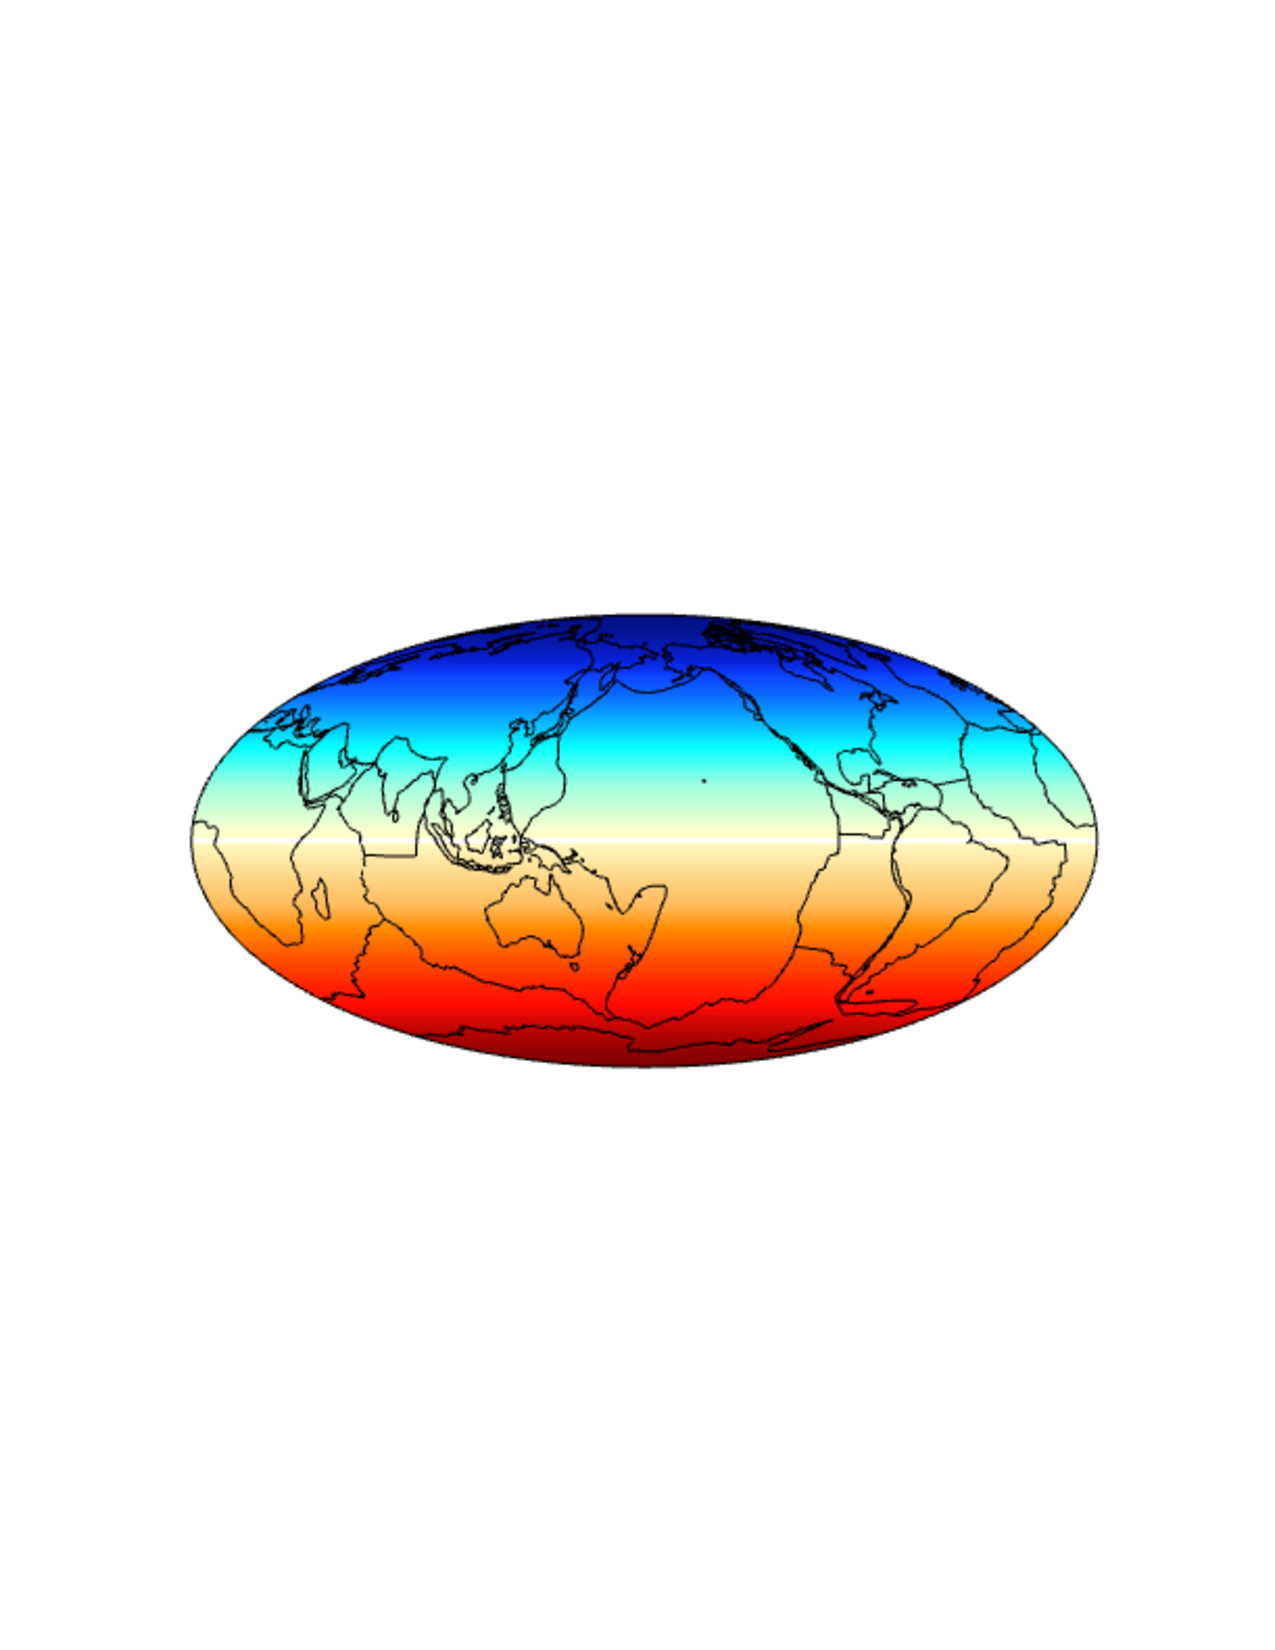
\includegraphics[width=0.4\textwidth,trim = 3cm 9cm 3cm 10cm, clip]{figures/Y10_Mol}
\caption{This is spherical harmonic $\Yfun_{1\,0}$. It's a dipole with its north pole over the geographical North Pole and its south pole over the geographical South Pole. In the left panel I am plotting it over a sphere, in the right panel I am using Mollweide projection}
\label{Y10fig}
\end{figure}

%\newpage
\begin{figure}[H]
\centering
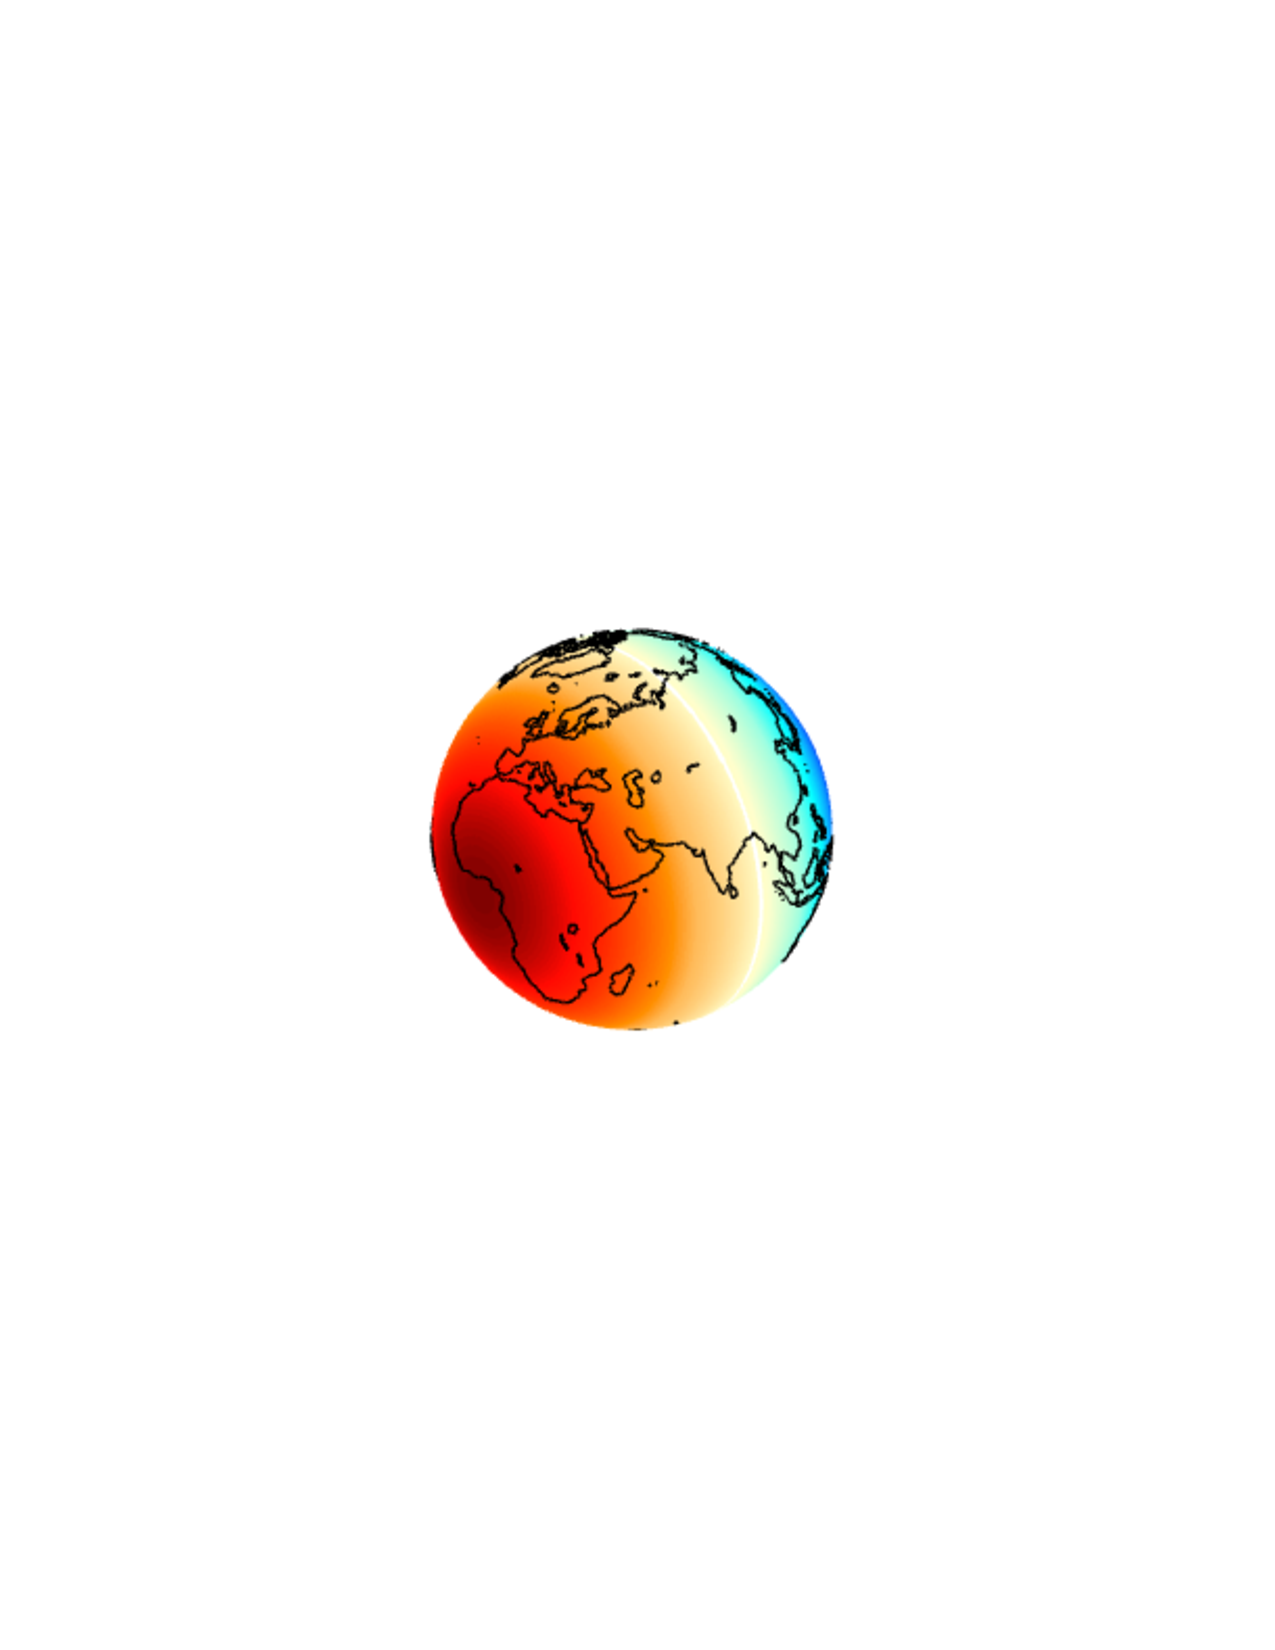
\includegraphics[width=0.4\textwidth,trim = 7cm 10cm 7cm 10cm, clip]{figures/Y1m1}
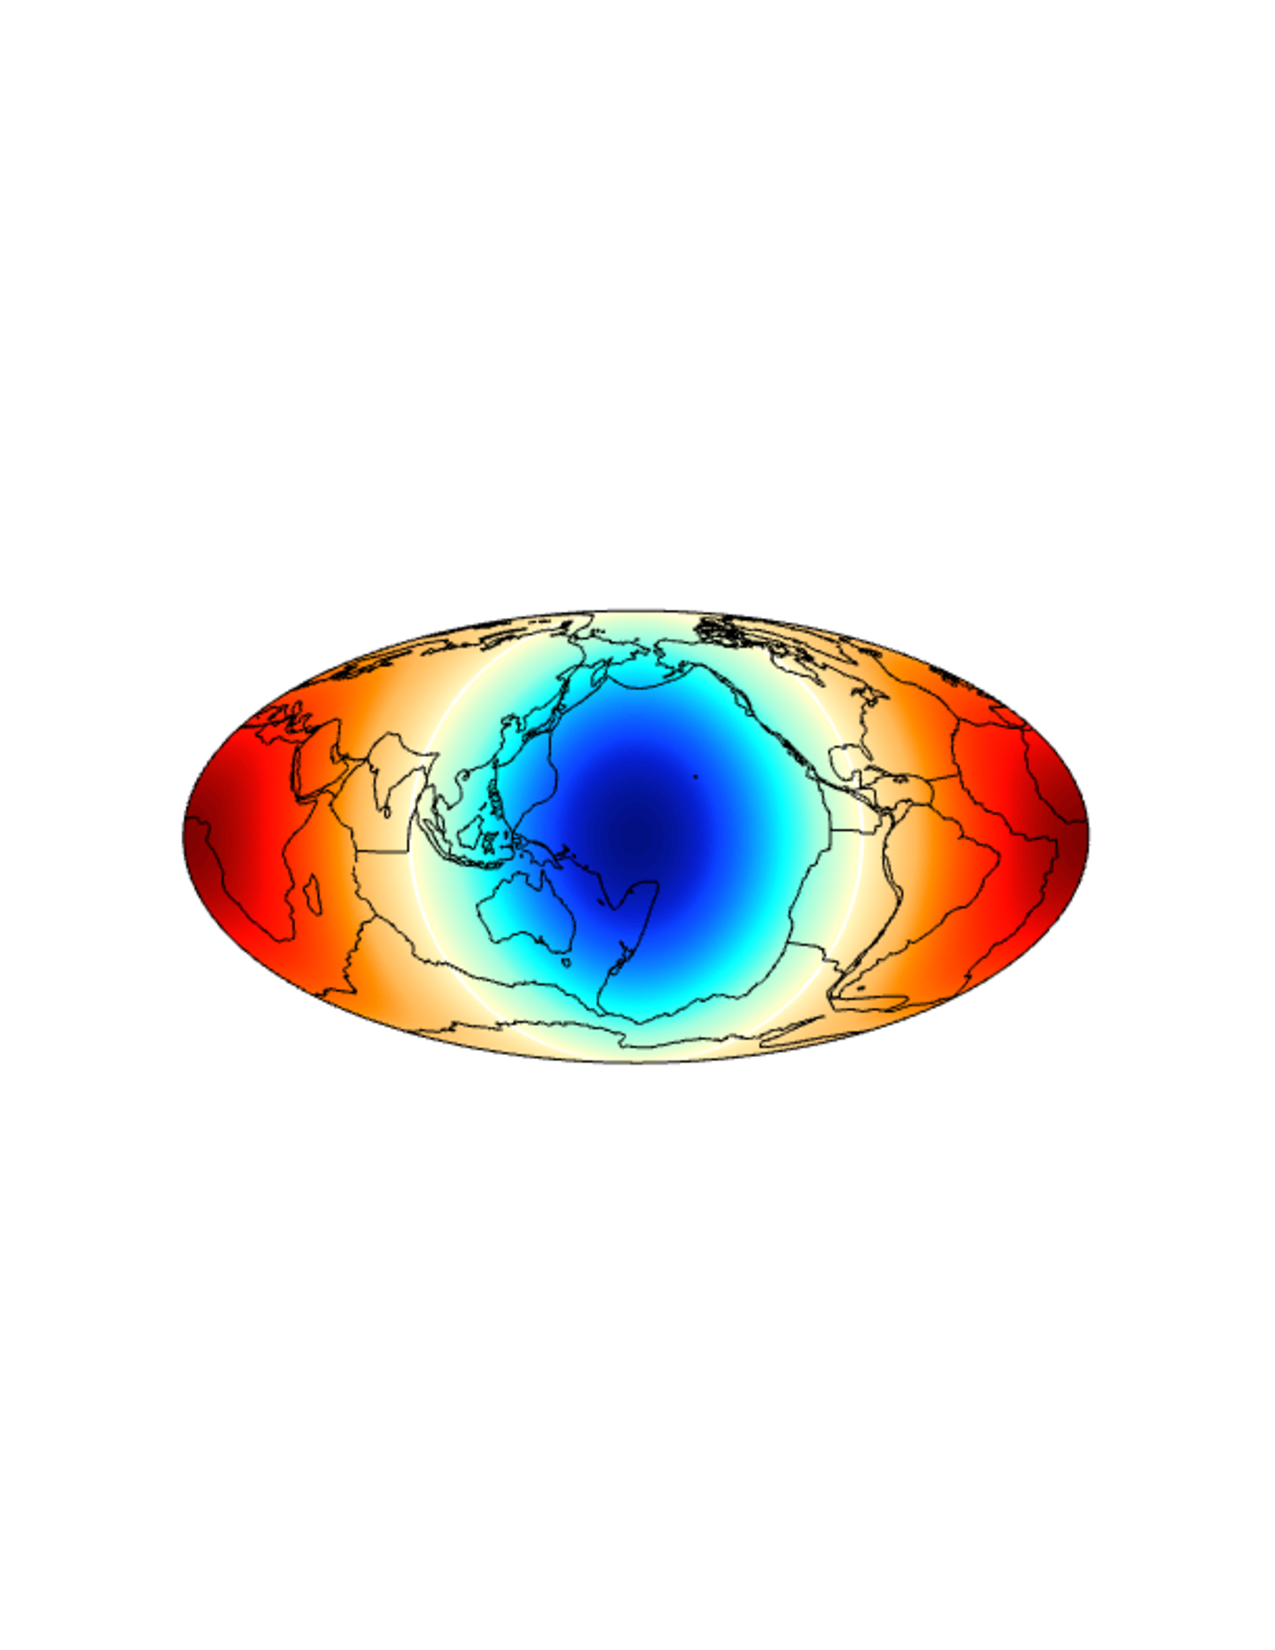
\includegraphics[width=0.4\textwidth,trim = 3cm 9cm 3cm 10cm, clip]{figures/Y1m1_Mol}
\caption{This is spherical harmonic $\Yfun_{1\,-1}$. It's a dipole with its north pole over the Pacific and its south pole over Africa. In the left panel I am plotting it over a sphere, in the right panel I am using Mollweide projection.}
\label{Y1m1fig}
\end{figure}
 
 \begin{figure}[h!]
\centering
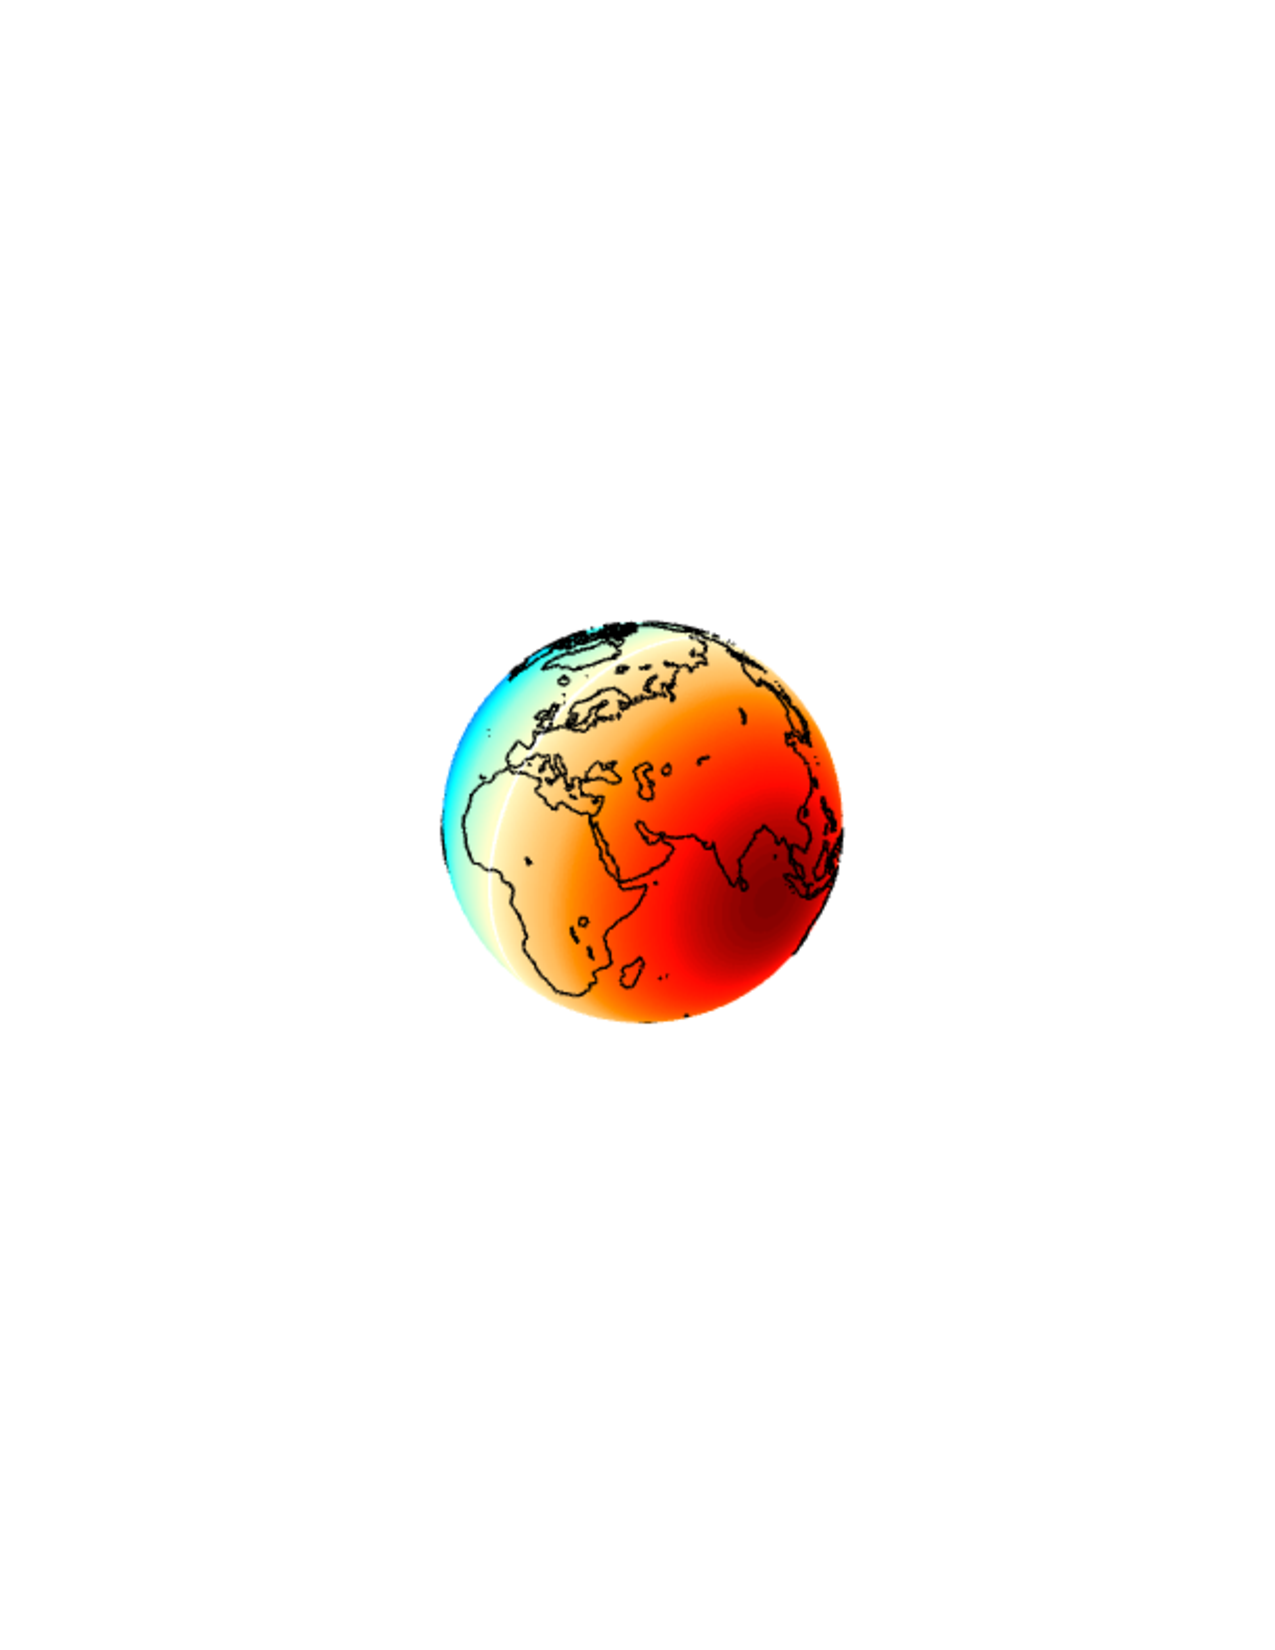
\includegraphics[width=0.4\textwidth,trim = 7cm 10cm 7cm 10cm, clip]{figures/Y11}
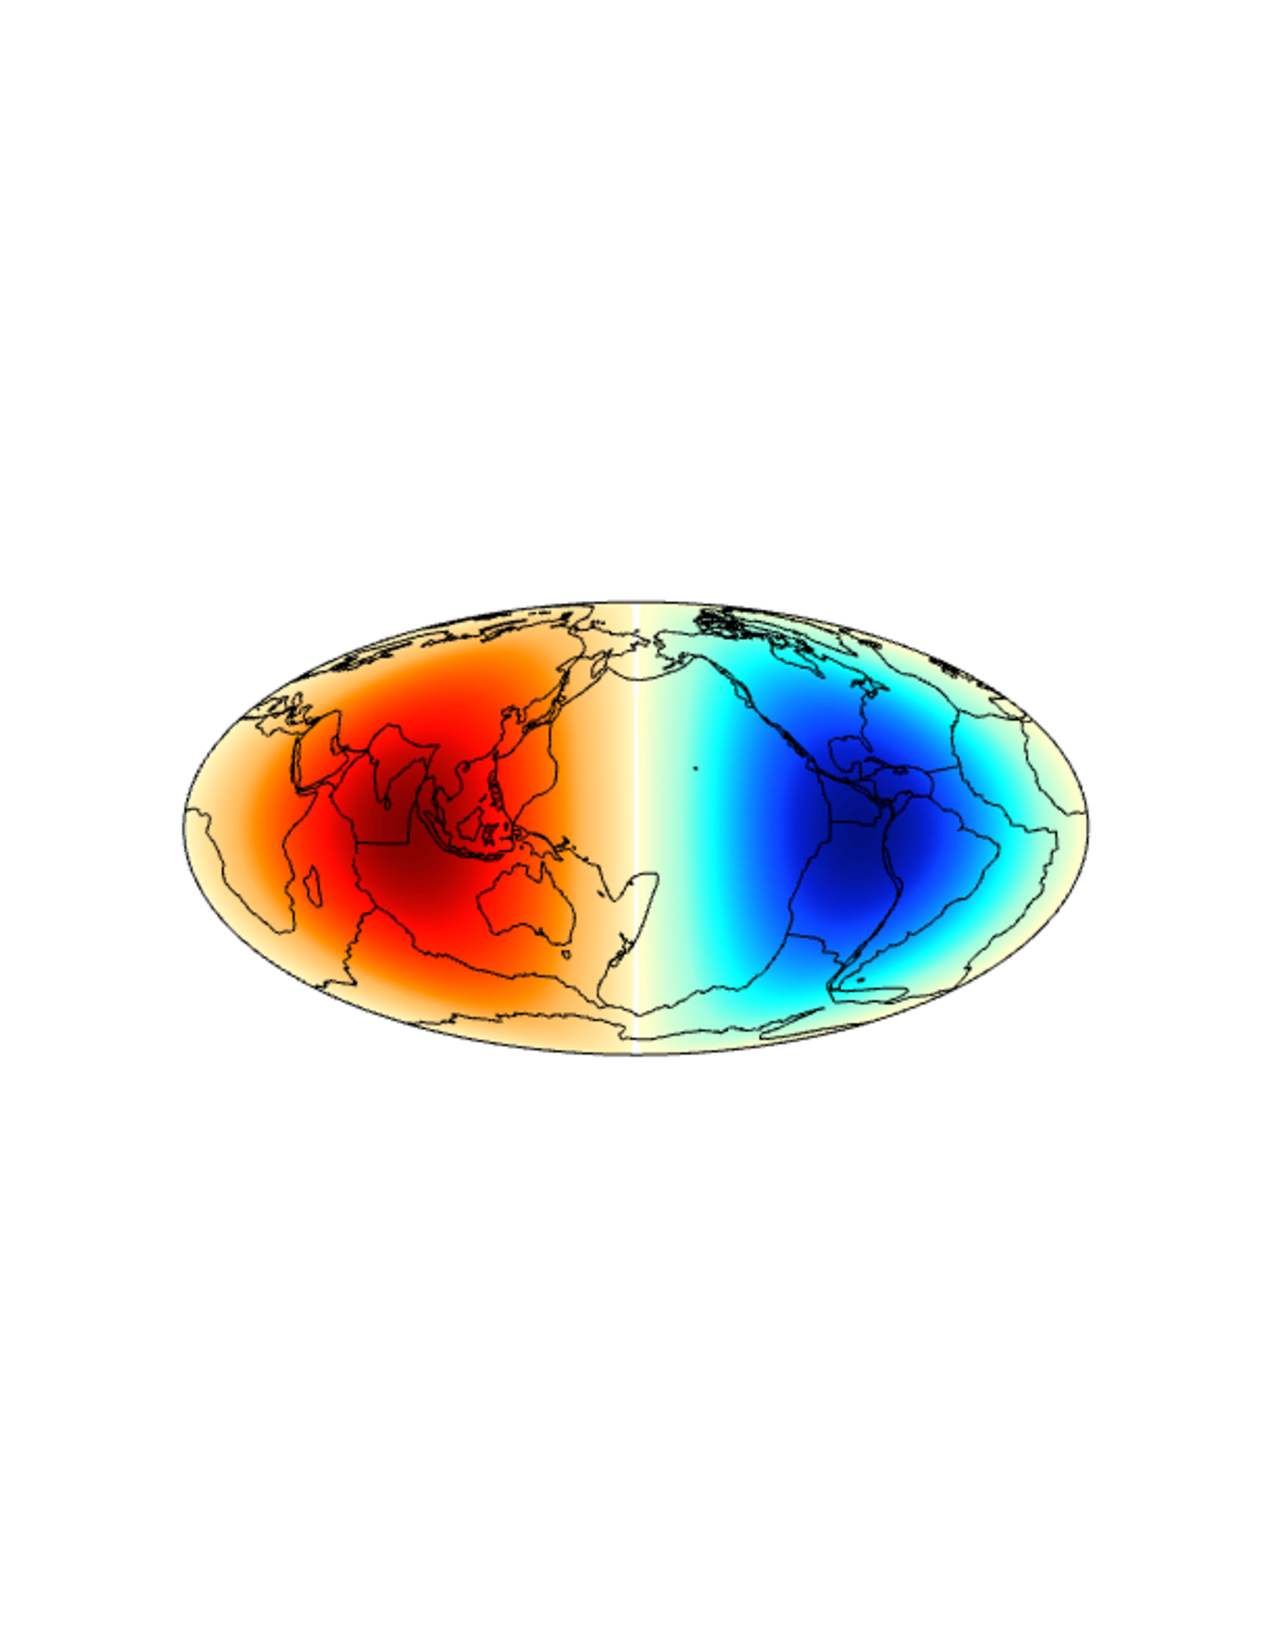
\includegraphics[width=0.4\textwidth,trim = 3cm 9cm 3cm 10cm, clip]{figures/Y11_Mol}
\caption{This is spherical harmonic $\Yfun_{1\,1}$. It's a dipole with its north pole over the Indian Ocean and its south pole over Central America. In the left panel I am plotting it over a sphere, in the right panel I am using Mollweide projection.}
\label{Y11fig}
\end{figure}
 
 \textbf{Question:} How can we make a dipole with its south pole over the geographical North Pole and its North pole over the geographical South Pole?
 
 
 I made these plots using our codes that you just installed. Once you chose a degree $l$ and an order $m$, you must select a plotting grid. Let's make a pixel every half degree. From your Octave tutorial you remember that 
  
\qquad \verb+theta=-90:0.5:90;+

Sets up such a vector for the latitudes and 

\qquad \verb+phi=-180:0.5:180;+

for the longitudes. We will use the function \verb+ylm.m+ to calculate spherical-harmonic values on the sphere on the grid we just defined. Notice that the symbol \verb+l+ is the letter $l$. Run

\qquad \verb+l=3+ 

and 

\qquad \verb+m=-2+

and then 

 \qquad \verb+Y3m2=ylm(l,m,pi/180*(90-theta),pi/180*phi);+
 
 This will calculate the values of $\Yfun_{lm}$ for your chosen $l$ and $m$ on the grid you defined with latitudes \verb+theta+ and longitudes \verb+phi+. We need the factors $\pi/180$ because the function \verb+ylm.m+ requires the grid in radians and we need the $90-$ \verb+theta+ because the function \verb+ylm.m+ works with colatitudes instead of latitudes.
 
  To plot the resulting evaluated spherical harmonic \verb+Y3m2+ on a Mollweide projection, run
 
 \qquad \verb+plotplm(Y3m2,pi/180*phi,pi/180*theta,1)+
 
Let's change the color to a bit a nicer color scheme, run
 
 \quad \verb+kelicol(1)+
 

To plot the resulting evaluated spherical harmonic on a rotatable sphere, you need to first open a new figure or close the old one and then run

 \qquad \verb+plotplm(Y3m2,pi/180*phi,pi/180*theta,2)+
 
 The Octave version on my computer had issues with using the \verb+print+ command to turn figures into pdfs. I needed to take screen shots to get these figures into the document. This bug will probably be fixed soon and might not occur on your computer.

\textbf{Exercise:} Reproduce figures \ref{Y10fig}, \ref{Y1m1fig}, and \ref{Y11fig}. Plot different spherical harmonics for different degrees and orders. Plot sums of spherical harmonics. Plot linear combinations of spherical harmonics. How does for example \\{$4\Yfun_{3\,1} - 0.2\Yfun_{1\,-1} +2\Yfun_{5\,-2}$} look like?

If it looks like in figure~\ref{MixY}, then your programing was correct.

\begin{figure}[H]
\centering
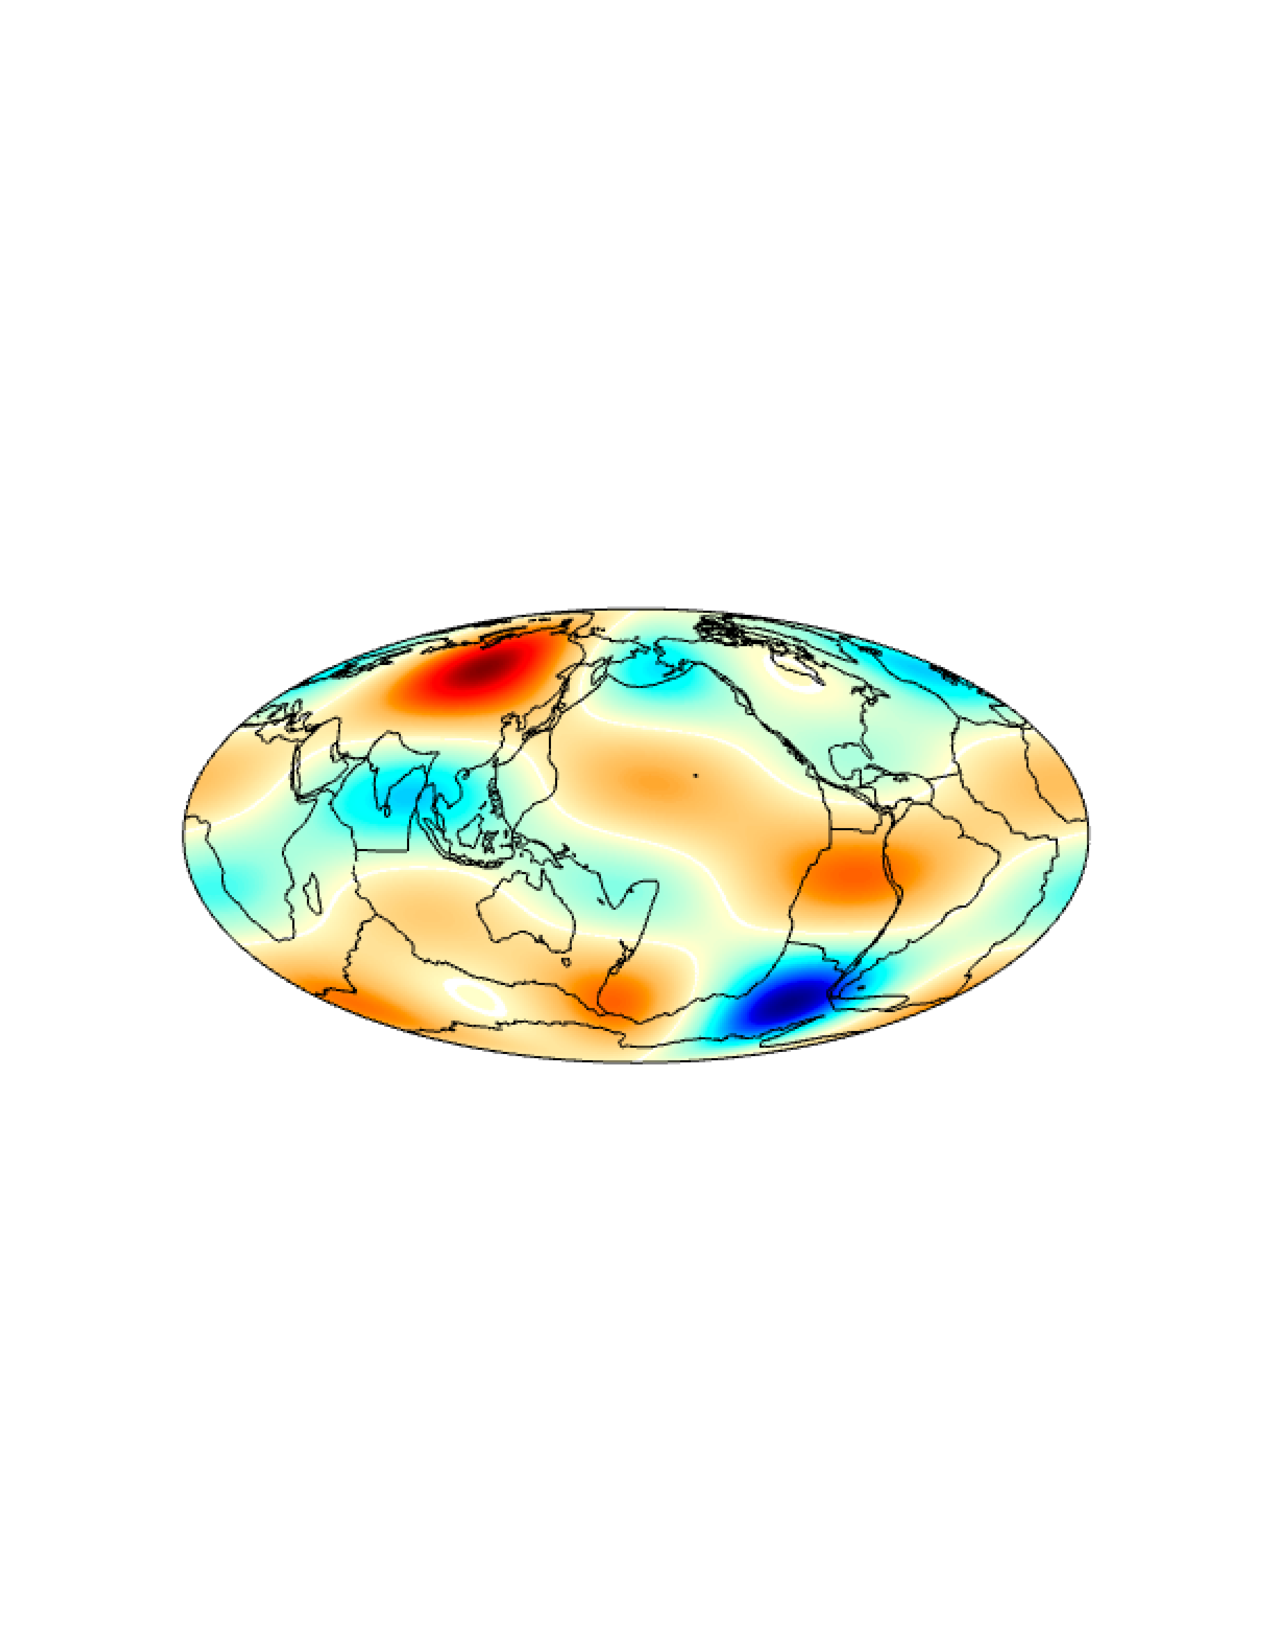
\includegraphics[width=0.7\textwidth,trim = 3cm 9cm 3cm 10cm, clip]{figures/mixY}
\caption{Linear combination of spherical harmonics $4\Yfun_{3\,1} - 0.2\Yfun_{1\,-1} +2\Yfun_{5\,-2}$ in Mollweide projection}
\label{MixY}
\end{figure}

What we learn from this is that even though the individual spherical harmonics look very regular with their zero-crossings either parallel or perpendicular to the equator, linear combinations of spherical harmonics can look very arbitrary. In fact, every reasonably behaved function on the sphere (no infinite values and no sudden jumps, etc.) can be expressed as a linear combination of spherical harmonics. For some we might need spherical harmonics with very high degrees.

\textbf{Exercise:} Make your own linear combination of spherical harmonics. Play around with the degrees and coefficients. Can you make up some shape in your mind that you want to draw with spherical harmonics and then reproduce it?

Calculating spherical harmonics individually, multiplying them with coefficients, and then summing them up is cumbersome. Luckily, our software allows us to do this more efficiently. Instead of just calculating a single spherical harmonic we can calculate all of them up to a any degree
 $L$ we choose. Run for example
 
  \quad \verb+L=10+
  
  and then
  
   \quad \verb+Y=ylm([0 L],[],pi/180*(90-theta),pi/180*phi);+
   
   This will calculate a matrix \verb+Y+ in which each row represents an evaluated spherical harmonic. the rows are ordered in what we call here the \emph{addmout} format. This is an informal term used within the software suite and is not generally used in the community. Addmout means the following ordering for the (degree/order) pairs: (0/0), (1/-1), (1/0), (1/1), (2/-2), (2/-1), etc. This means that the spherical harmonic with degree 2 and order 1 is in the 8th row of the matrix \verb+Y+. 
   
   \textbf{Question:} In which row is degree 3, order -2? Which degree/order pair do we find in row 20?
   
   If we now have a vector of coefficients that we call \verb+c+, then we can calculate the linear combination of the spherical harmonics evaluated in matrix \verb+Y+ with the coefficients in vector \verb+c+ using matrix-vector multiplication. For a maximum spherical harmonic degree $L$ there are $(L+1)^2$ spherical harmonics including all degrees between 0 and $L$ and all corresponding orders. 
   We can calculate a random row vector with the correct length by running
   
   \quad \verb!c=randn(1,(L+1)^2);!
   
   and evaluate the linear combination of the spherical harmonics as
   
    \quad \verb!F=c*Y;!
   
   The linear combination \verb!F! has the form of a vector. We need to put it into the right shape by running 
   
   \quad \verb!Fp=reshape(F,length(theta),length(phi));!
   
   Plot this function with the command we have seen before
   
    \qquad \verb+plotplm(Fp,pi/180*phi,pi/180*theta,1)+
   
   \textbf{Question:} Why are there $(L+1)^2$ spherical harmonics for degrees 0 to $L$ and all coprresponding orders?
   
   \textbf{Question:} Why does the matrix vector multiplication \verb!F=c*Y;! calculate a linear combination of the spherical harmonics with the corresponding coefficients in \verb+c+?
   
   
   \textbf{Exercise:} If I give you a random list of data point values together with their locations, can you find a way to calculate best-fitting spherical-harmonic coefficients? Remember least-squares fitting. 
   
   
   
   
    
   
 
   
  


\end{document}